\listfiles

\documentclass[11.5pt,a4paper]{article}

\usepackage{amsthm,amssymb,amsmath}

\usepackage{mathtools}

\newcommand\persiangloss[2]{#1\dotfill\lr{#2}\\}

\newcommand{\nocontentsline}[3]{}
\newcommand{\tocless}[2]{\bgroup\let\addcontentsline=\nocontentsline#1{#2}\egroup}
\usepackage[bottom]{footmisc}
\usepackage{indentfirst}

\usepackage{caption}

\usepackage{graphicx}
\usepackage{subcaption}
\usepackage{array}
\usepackage{adjustbox}
\usepackage{tablefootnote}
\usepackage{amsfonts}
\usepackage{amssymb}
\usepackage{yfonts}

\usepackage[scr=euler,bb=ams]{mathalfa}

\usepackage{xcolor,colortbl}
\definecolor{Gray}{gray}{0.90}
\definecolor{LGray}{gray}{0.95}

\usepackage[pagebackref=false,colorlinks,linkcolor=blue,citecolor=magenta]{hyperref}

\usepackage{xepersian}
\settextfont[Scale=1]{Persian Modern}
\setlatintextfont[Scale=1]{Latin Modern Roman}

%\settextfont[Scale=1.1]{B Zar}

%\DefaultMathsDigits
\setdigitfont{Persian Modern}

\defpersianfont\titr[Scale=1]{B Titr}
%\defpersianfont\nastaliq[Scale=1.5]{IranNastaliq}
%\defpersianfont\traffic[Scale=1]{B Traffic}
%\defpersianfont\yekan[Scale=1]{B Yekan}
%\defpersianfont\traffic[Scale=1]{XB Roya}
%\defpersianfont\yekan[Scale=1]{XB Kayhan}
%%%%%%%%%%%%%%%%%%%%%%%%%%%%%%%%%%%%%%%%%%%%%%%%%%%
\usepackage{zref-perpage}
\zmakeperpage{footnote}


\begin{document}

\thispagestyle{empty}
\vspace*{-28mm}
\centerline{
\includegraphics[height=5cm]{logo.png}}

\begin{center}
%دستوری برای کم کردن فاصله بین لوگو و خط پایین آن
\vspace{-2mm}
{\large
گروه مستقل مهندسی رباتیک
%دستوری برای تعیین فاصله بین دو خط
\\[2.1cm]
}

{\large
\textbf{گزارش تمرین اول درس مدل‌های احتمالاتی گرافی}
\\[2cm]

استاد درس:
\\[.5cm]
{\Large
دکتر نیک‌آبادی}
\\[1.5cm]
\large 
تدریس‌یار:
\\[.5cm]
{\Large
مهندس طاهرخانی}
\\[1.5cm]

\large 
نام دانشجو:
\\[.5cm]
{\Large
نوید خزاعی}
\\[.5cm]
۹۲۱۳۵۰۰۸
\\[1.5cm]
}
%دستوری برای تعیین فاصله بین خطوط (نه دو خط) و تا وقتی که مقدار آن تغییر نکند، فاصله بین خطوط، همین مقدار است.

{\large
اردیبهشت ۹۴
}
\end{center}

\newpage
\baselineskip=1cm
\tocless\tableofcontents

\newpage
\baselineskip=0.75cm
\pagenumbering{arabic}
\section{بخش نظری}
\subsection{سوال اول}
قضیه زیر را اثبات کنید: 
\begin{latin}
\lr{
\emph{Theorem 1. Let $\mathcal{G}$ be a Bayesian Network structure over a set of random variables $\mathcal{X}$ and let $\mathit{P}$ be a joint distribution over $\mathcal{X}$. If $\mathit{P}$ factorizes according to $\mathcal{G}$, then $\mathcal{G}$ is an  $\mathit{I}$-map for $\mathit{P}$}.}
\end{latin}

پاسخ: 

با توجه به این که $\mathit{P}$ روی گراف $\mathcal{G}$ فاکتورایز می‌شود، پس می‌دانیم که: 
\begin{equation}
P (X_1 , \dots , X_n ) = \prod_{i=1}^n P (X_i \ | \ \text{\lr{Pa}}(X_i )),
\label{eq1}
\end{equation}

که در آن 
$\mathit{\text{\lr{Pa}}(X_i)}$ 
والدین متغیر تصادفی 
$\mathit{i}$
م هستند. برای آن که نشان‌دهیم گراف $\mathcal{G}$ یک 
\lr{ $\mathit{I}$-$\mathit{map}$}
برای 
$\mathit{P}$
است، باید نشان‌دهیم 
$\mathit{I}(\mathcal{G}) \subseteq \mathit{I}(\mathcal{P})$
. با توجه به آن‌چه در درس آمده بود، اگر مجموعه روابط استقلال 
$\mathit{I}(\mathcal{G})$
را به‌گونه‌ای با استفاده از نتایج فرمول \ref{eq1} نشان‌ دهیم، یعنی این روابط از روابط استقلال توزیع مورد نظر استخراج شده‌اند پس زیرمجموعه‌ی آن نیز هستند. برای این کار، با توجه به این که مجموعه روابط استقلال در گراف ایجاب می‌کند که: 
\begin{equation}
\lbrace X_{i} \perp \text{\lr{ND}}(X_{i}) \ | \ \text{\lr{Pa}}(X_i); i = 1, \dots , n \rbrace
\label{eq2}
\end{equation}

که در آن
$\text{\lr{ND}}(X_{i})$
مجموعه‌ی غیرنسل\LTRfootnote{ Non-descendant} متغیر 
$\mathit(X_{i})$
است. اگر بتوانیم نشان‌دهیم که :
\begin{equation}
P(X_{i} \ | \ \text{\lr{ND}}(X_{i})) =  P(X_{i} \ | \ \text{\lr{Pa}}(X_i))
\label{eq3}
\end{equation}
آن‌گاه رابطه‌ی استقلال \ref{eq2} برقرار است. برای این‌کار 
$P(X_{i} \ | \ \text{\lr{ND}}(X_{i}))$
را محاسبه می‌کنیم (نسل 
$X_i$
با 
$\text{\lr{D}}(X_i)$
نشان داده شده‌است) : 
\begin{spreadlines}{15pt}  
\begin{equation}
\begin{split}
{P(X_{i} \ | \ \text{\lr{ND}}(X_{i}))} & = {{P(X_{i} , \text{\lr{ND}}(X_{i}))} \over {P(\text{\lr{ND}}(X_{i}))} } = { {\sum_{\text{\lr{D}}(X_i)} P(X_1 , \dots , X_n)} \over {\sum_{X_i , \text{\lr{D}}(X_i)} P(X_1 , \dots , X_n)} } \\ 
	& = { {\sum_{\text{\lr{D}}(X_i)} \prod_{j=1}^{n}P(X_j\ | \ {\text{\lr{Pa}}(X_j)})} \over {\sum_{X_i, \text{\lr{D}}(X_i) } \prod_{j=1}^{n}P(X_j\ | \ {\text{\lr{Pa}}(X_j)})} }
\end{split}
\label{eq4}
\end{equation}
\end{spreadlines}
در \ref{eq4} در محاسبه‌ی سیگما، مواردی هستند که جزو نسل 
$X_i$
نیستند، پس می‌توان آن‌ها را از سیگمای روی نسل آن خارج نمود. همچنین آن‌چه باقی می‌ماند:
\begin{equation*}
{\sum_{\text{\lr{D}}(X_i)} \ \prod_{X_j \in {\text{\lr{D}}(X_i)}}P(X_j\ | \ {\text{\lr{Pa}}(X_j)})} = 1
\end{equation*}

مشابه همین استدلال برای مخرج نیز پاسخ‌گو است، لذا خواهیم داشت: 
\begin{spreadlines}{15pt}  
\begin{equation}
\begin{split}
\phantom{nothing} & = { {\prod_{X_j \in ( \text{\lr{ND}}(X_i) \cup X_i ) } P(X_j \ | \ \text{\lr{Pa}}(X_j)) \times 1 } \over {\prod_{X_j \in \text{\lr{ND}}(X_i) } P(X_j \ | \ \text{\lr{Pa}}(X_j)) \times 1 } } \\
	& = P(X_i \ | \ \text{\lr{Pa}}(X_i) ).
\end{split}
\end{equation}
\end{spreadlines}

پس نشان‌دادیم \ref{eq3} و در نتیجه \ref{eq2} برقرار است، پس می‌توان نتیجه گرفت که $\mathit{I}(\mathcal{G}) \subseteq \mathit{I}(\mathcal{P})$، و حکم اثبات می‌شود. 

\subsection{سوال دوم}
با توجه به شبکه‌ی شکل \ref{fig1} به سوالات پاسخ داده شده‌است.
\begin{figure}[h]
\centering
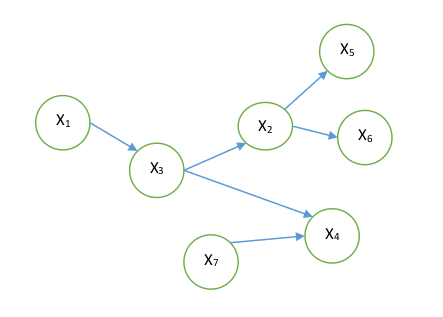
\includegraphics[width=0.5\textwidth]{4}
\caption{شکل سوال دوم}
\label{fig1}
\end{figure}

\subsubsection{توزیع توام}

$P(X_1, \dots , X_7) = P(X_1)P(X_3 \ | \ X_1)P(X_2 \ | \ X_3)P(X_5 \ | \ X_2)P(X_6 \ | \ X_2)P(X_4 \ | \ X_3 , X_7)P(X_7)$

\subsubsection{درستی و نادرستی}

\begin{itemize}
\item{$X_1 \perp X_5 \ | \ X_2 $}:
درست است. اگر 
$X_2$
را بدانیم مسیر فعال بین $X_1$ و $X_5$ غیر فعال می‌شود و مستقل می‌شوند.
\item{$X_2 \perp X_7 \ | \ X_4 $}:
نادرست است. در ساختار وی-شکل بین $X_7$ و $X_3$ با دانستن $X_4$ وابستگی ایجاد می‌شود، و چون $X_2$ به پدرش $X_3$ وابسته است، با $X_7$ نیز در این شرایط وابسته است. 

\item{$X_1 \perp X_5 \ | \ X_2 $}:
درست است، چرا که دانستن $X_3$ ، استقلال بین $X_2$ و $X_4$ را ایجاد می‌کند و بنابر این از فرزندان $X_2$ یعنی $X_5$ نیز مستقل می‌شویم. 

\subsubsection{ \lr{Markov Blanket for $X_3$} }
برای این کار ابتدا جهت‌ها را حذف می‌کنیم و سپس فساد\LTRfootnote{ Immorality} ها را حذف می‌کنیم. یعنی نباید گره‌ای باشد که والد یکی از فرزندان همین گره باشد، در صورت وجود به آن گره وصل می‌کنیم تا فساد از بین برود. به تمامی اتصالات موجود نیز وصل می‌کنیم، بنا بر این
$MB(X_3) = \lbrace X_1 , X_2 , X_4 , X_7 \rbrace $
خواهد بود. 
\end{itemize}

\section{بخش پیاده‌سازی}















\end{document} 
